\documentclass{article}
\usepackage[final]{neurips}
\usepackage[framemethod=tikz]{mdframed}
\usepackage{lipsum}
\definecolor{mycolor}{rgb}{0.122, 0.435, 0.698}
\newmdenv[innerlinewidth=0.5pt, roundcorner=4pt,linecolor=mycolor,innerleftmargin=6pt,
innerrightmargin=6pt,innertopmargin=6pt,innerbottommargin=6pt]{mybox}
\usepackage[utf8]{inputenc} % allow utf-8 input
\usepackage[T1]{fontenc}    % use 8-bit T1 fonts
\usepackage[hidelinks]{hyperref}       % hyperlinks
\usepackage{url}            % simple URL typesetting
\usepackage{booktabs}       % professional-quality tables
\usepackage{amsfonts}       % blackboard math symbols
\usepackage{nicefrac,tcolorbox}       % compact symbols for 1/2, etc.
\usepackage{amsmath}
\usepackage{enumitem}
\usepackage{microtype}      % microtypography
\usepackage{graphicx,caption,fontspec}
\usepackage{xepersian}
\settextfont{XB Niloofar}
\setdigitfont{XB Niloofar}
\raggedbottom


\title{
	\vspace{-0.8em}
تمرین امتیازی 1 - درس نظریه گروه‌ها - دکتر رضاخانی
\\
{\normalsize
\textbf{مهلت تحویل:
نزدیک‌ترین زمان از بین پایان‌کلاس‌ها و موعد آخرین سری تمرین‌ها
\\
\vspace{-0.4em}
از طریق سامانه
\href{https://cw.sharif.edu/}{درس‌افزار شریف}
}
}
\vspace{-0.6em}
}

\usepackage[utf8]{inputenc}

\usepackage[english]{babel}
\setlength{\parindent}{3.5em}
\setlength{\parskip}{0.5em}
\renewcommand{\baselinestretch}{1.0}

\usepackage{calrsfs}
\DeclareMathAlphabet{\pazocal}{OMS}{zplm}{m}{n}
\newcommand{\La}{\mathcal{L}}
\newcommand{\Lb}{\pazocal{L}}

\newtcolorbox{boxes}[3][]
{
	colframe = #2!25,
	colback  = #2!10,
	coltitle = #2!40!black,  
	title    = {\textbf{#3}},
	#1,
}

\newenvironment{exercise}[3][\unskip]{%
	\par
	\noindent
	\textbf{تمرین
		#1
		[#2 امتیاز] 
		\def\temp{#3}\ifx\temp\empty
		: 
		\else
		: #3 \vspace{0.5em} \\ \noindent
		\fi
}}{}

\author{
حسین محمدی\\
  \lr{
  		\href{mailto:hossein.mohammadi.00427@gmail.com}{\texttt{	hossein.mohammadi.00427@gmail.com}}} \\
  \And
  زهرا کبیری\\
 \lr{
  		\href{mailto:kabiri.zahra98@gmail.com}{ \texttt{kabiri.zahra98@gmail.com}}}\\
  }

\begin{document}


\begin{minipage}{0.1\textwidth}% adapt widths of minipages to your needs
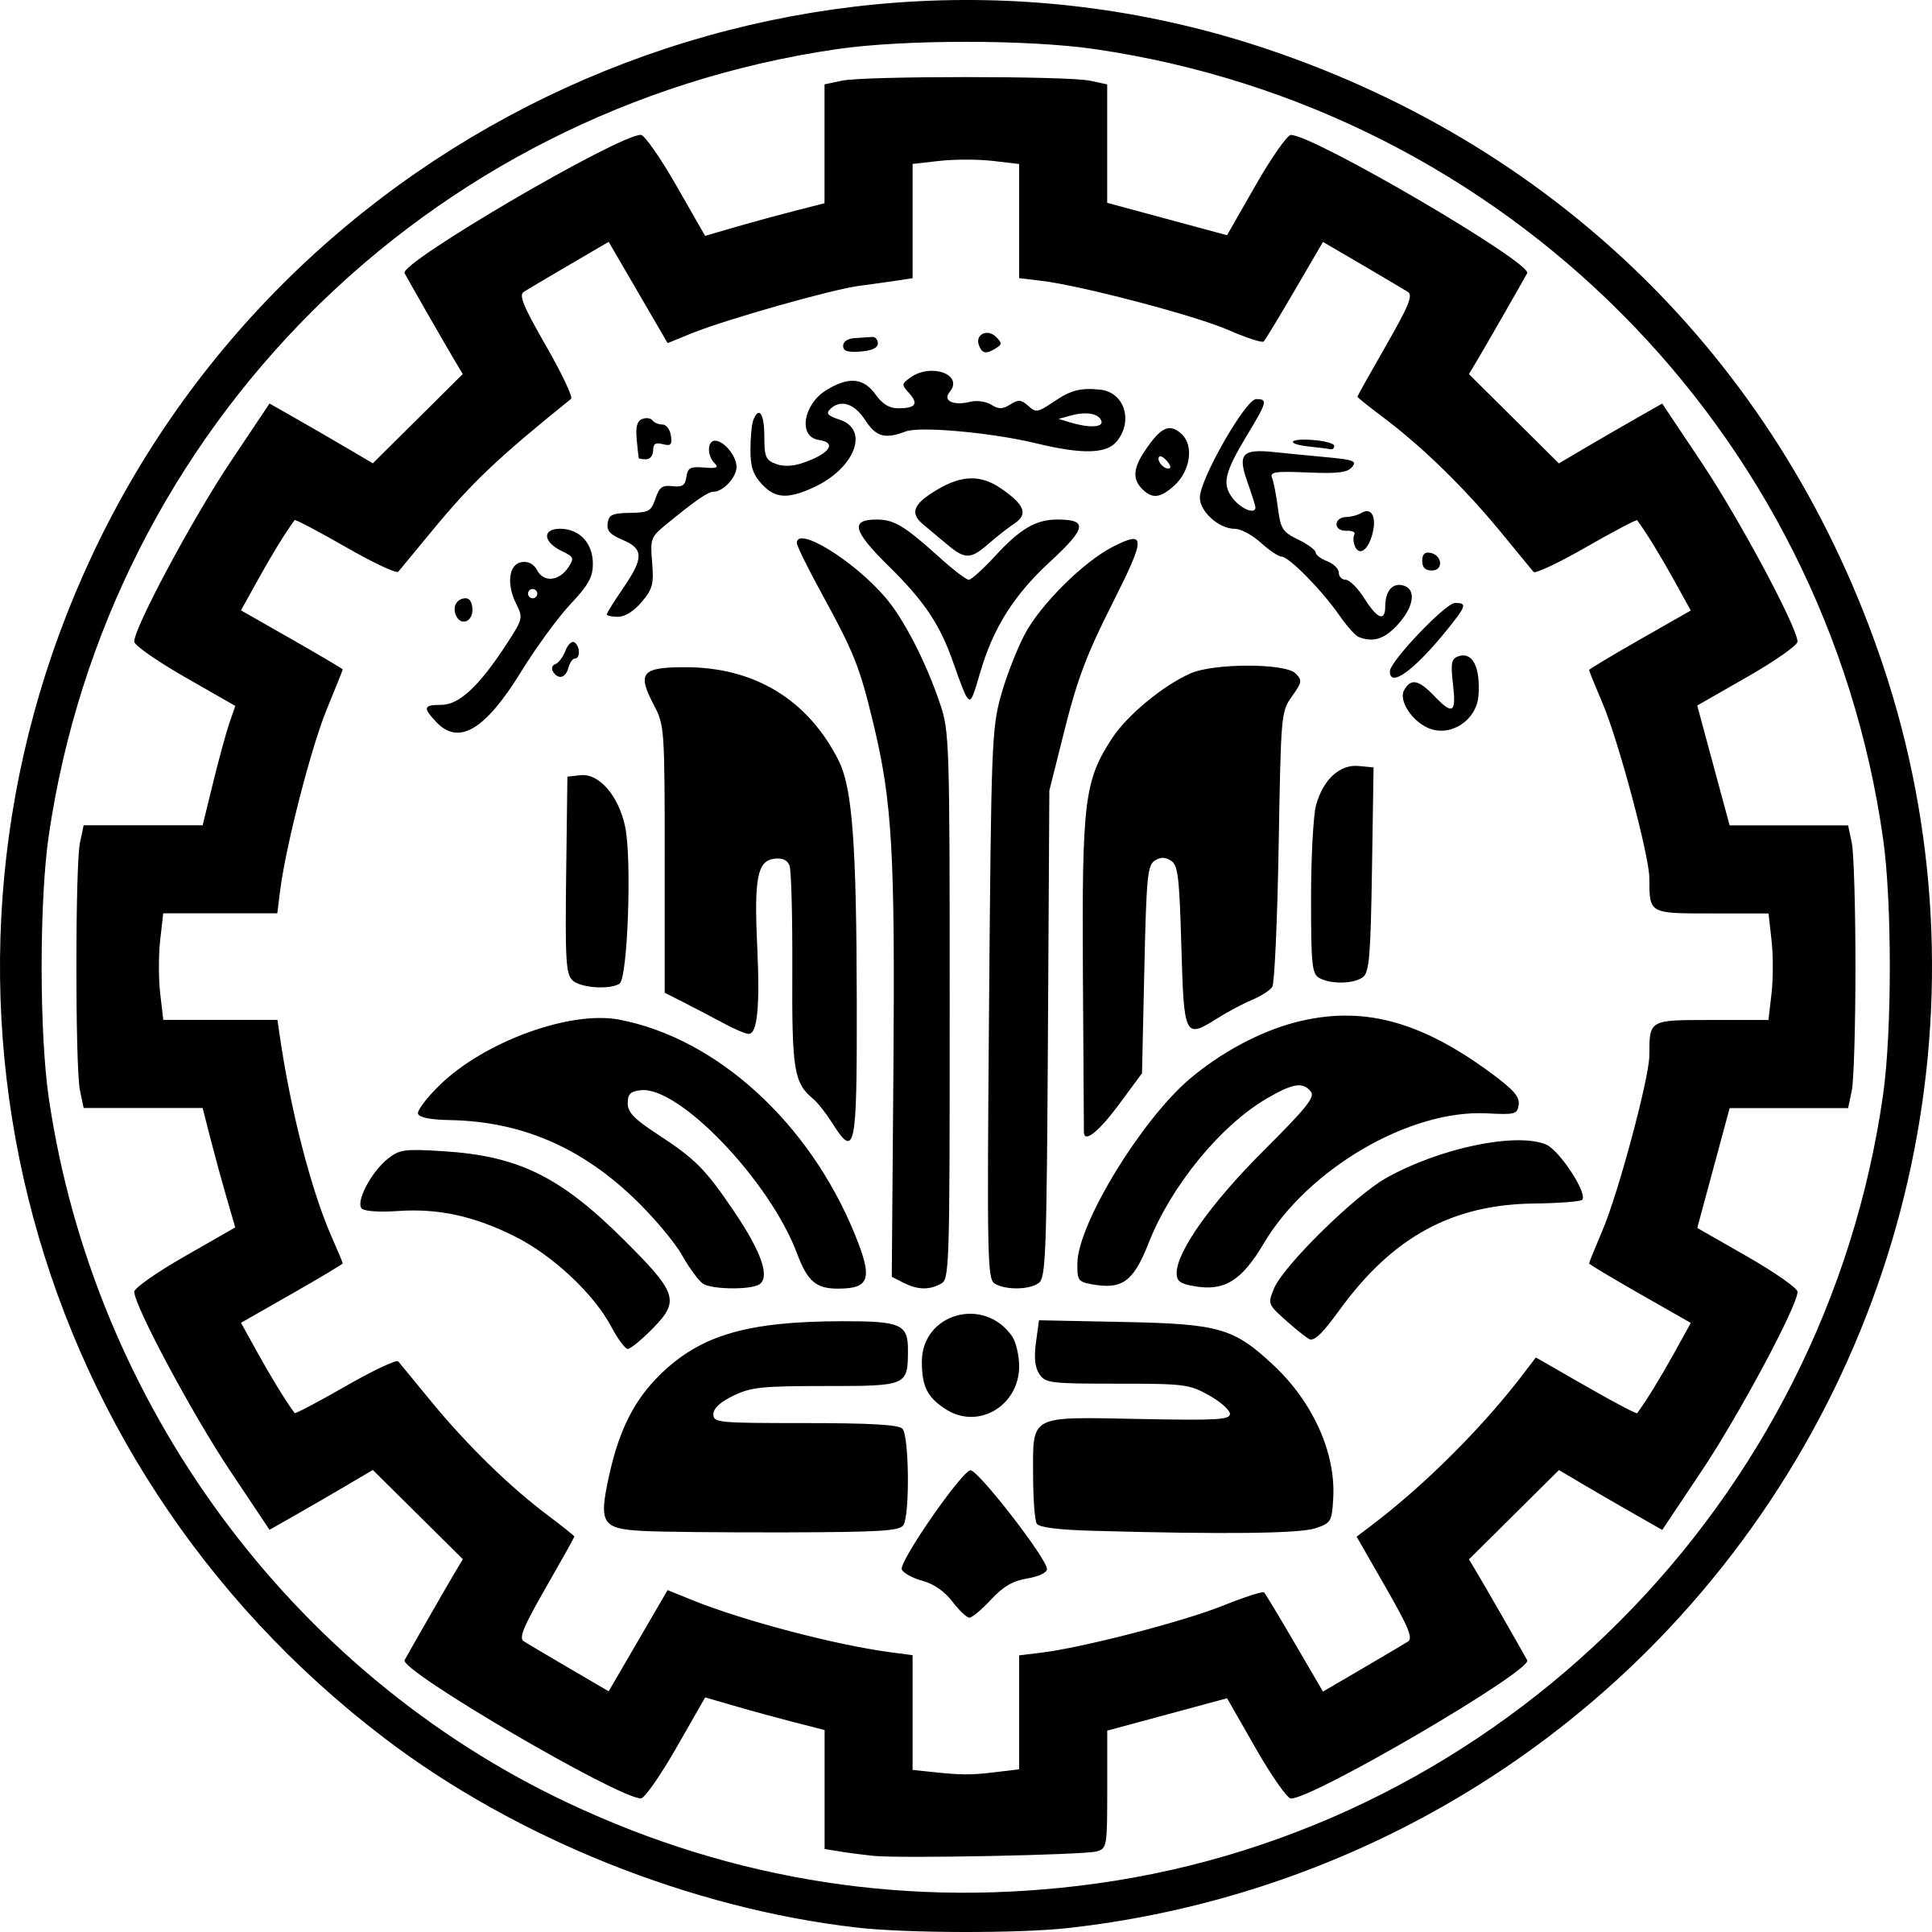
\includegraphics[width=1.1cm]{sharif-logo.png}
\end{minipage}%
\hfill%
\begin{minipage}{0.9\textwidth}\raggedleft
دانشگاه صنعتی شریف\\
زمستان ۱۴۰۲ - بهار ۱۴۰۳\\
\end{minipage}

\makepertitle

\noindent
برای جبران نمرات از دست رفته، به حل سوالات امتیازی بپردازید. با این شرایط که:
\begin{enumerate}
	\item برای کسب نمره‌ی کامل، دو سوال را  از دسته‌ی اول و چهار سوال را از دسته‌ی دوم انتخاب و حل کنید. 
	\item در مورد سوالات چندبخشی، حل باید به ترتیب انجام بگیرد و نمی‌توان بدون حل یک قسمت، از نتیجه‌اش در قسمت‌های بعدی استفاده کرد. 
	
\end{enumerate}

\section*{
	\LARGE
	دسته‌ی اول}

\begin{exercise}[$1''$]{20}{قضیه‌ی کوشی و قضیه کوچک فرما}
	الف) فرض کنید 
	$G$ گروهی مرتبه 
	$n$ باشد و 
	$p$
	عددی اول باشد. زیرمجموعه‌ی $S$ از مجموعه‌ی
	$\underbrace{G\times \dots \times G}_{p \; \text{times}} $
	را به این شکل تعریف کنید:
	\[
	S = \{(g_1,\dots,g_p) \; \big| \; g_1\dots g_p =e\}
	\]
	نشان دهید که
	\footnote{از آقای طالبی برای تذکر اشکال در سوال ممنونیم.} 
	\[
	|S| = n^{p-1}
	\]
	
	\noindent
	ب) با کمک قسمت قبل قضیه کوشی
	\LTRfootnote{Cauchy's Theorem}
	را ثابت کنید. 
	\begin{mdframed}
		اگر $G$ گروهی متناهی باشد و $p$ عددی اول که 
		$p \;| \;|G|$
		، آنگاه گروه $G$ عضوی از مرتبه $p$ دارد.
	\end{mdframed}
	
	\noindent
	ج) 
	\href{https://fa.wikipedia.org/wiki/%D9%82%D8%B6%DB%8C%D9%87_%DA%A9%D9%88%DA%86%DA%A9_%D9%81%D8%B1%D9%85%D8%A7}{قضیه کوچک فرما}
	را نیز ثابت کنید.
\end{exercise}

\begin{exercise}[$2''$]{-}{ }
	گروهی متناهی، $G$، و زیرگروه بهنجاری از آن ،$H$، مثال بزنید که 
	\[
	|\text{Aut}\; (H)| > |\text{Aut}\; (G)|
	\]
\end{exercise}

\begin{boxes}{black}{تعریف نیم‌گروه و تکواره}
	یک نیم‌گروه
	\LTRfootnote{Semigroup}
	، مجموعه‌ای چون
	$S$
	با عملی دوتایی شرکت پذیر است. لازم نیست سایر شرایط گروه در تعریف نیم‌گروه برقرار باشند.
	
	هم‌چنین تکواره 
	\LTRfootnote{Monoid}
	، یک نیم‌گروه است که عضو خنثای  چپ و راست هم دارد.
\end{boxes}


\begin{exercise}[$3''$]{-}{ }
	فرض کنید 
	$S$ یک نیم‌گروه باشد. نشان دهید شرایط زیر معادلند:
	\begin{enumerate}
		\item برای هر 
		$a,b\in S$
		معادلات 
		$ax=b$
		و
		$ya=b$
		با متغیرهای 
		$x,y \in S$
		دارای جواب هستند.
		\item $S$ دارای عضو خنثی است و هر عضو آن وارون‌پذیر است.
		\item برای هر 
		$a,b\in S$
		معادلات 
		$ax=b$
		و
		$ya=b$
		با متغیرهای 
		$x,y \in S$
		دارای جواب یگانه هستند.
		\item توابع ضرب از چپ
		$\lambda_s: S \longmapsto S$
		و ضرب از راست
		$\rho_s: S \longmapsto S$
		که با روابط 
		$\lambda_s(x) = sx$
		و 
		$\rho_s(x) = xs$
		معرفی‌ شده‌اند؛ برای هر 
		$s\in S$
		دوسویی اند.
	\end{enumerate}
\end{exercise}

\begin{exercise}[$4''$]{-}{ }
	الف)
	فرض کنید 
	$\phi: G\longmapsto G'$
	همریختی گروهی باشد و به علاوه زیرگروه‌های بهنجار 
	$N\trianglelefteq G$
	و
	$N' \trianglelefteq G'$
	مفروض‌اند. قرار دهید 
	$H = \phi^{-1}(N')$
	.
	نشان‌دهید که
	\[
	G/NH \simeq \text{im} (\phi) N' / \phi(N)N'
	\]
	
	\noindent
	ب)
	فرض کنید $H$ و $K$ دو زیرگروه بهنجار از $G$ باشند. ثابت کنید:
	\begin{enumerate}
		\item 
		$G/H\cap K $
		در
		$G/H \times G/K$
		می‌نشیند.
		\item اگر
		$HK=G$
		آنگاه
		$G/H\cap K \simeq G/H \times G/K$.
		\item 
		اگر 
		$[G:H]$
		و
		$[G:K]$
		متناهی و نسبت به‌هم اول باشند، آنگاه
		$G/H\cap K \simeq G/H \times G/K$.
	\end{enumerate}
\end{exercise}

\begin{exercise}[$5''$]{-}{ }
	الف) در گروه‌های 
	$S_{12}$
	و 
	$A_{17}$
	بیشینه مرتبه اعضا چیست؟
	
	\noindent
	ب)نشان دهید که 
	$A_5$ زیرگروه‌هایی با شاخص 
	۱۰ و ۶ دارد؛ 
	اما زیرگروه با شاخص ۳و۴ ندارد.
\end{exercise}
\section*{
	\LARGE
	دسته‌ی دوم}

\begin{exercise}[$6''$]{20}{}
	ثابت کنید که برای 
	$n>1$،
	گروه 
	$S_n$ با هیچ زیرگروهی از 
	$A_{n+1}$
	یکریخت نیست.
	
\end{exercise}


\begin{exercise}[$7''$]{20}{}
	نشان دهید که یک گروه متناهی دوری است اگر و فقط اگر از تمامی مراتبی که مقسوم‌علیه مرتبه‌ی آن هستند، یک زیرگروه یکتا داشته باشد. نتیجه بگیرید که برای هر عدد طبیعی $n$ داریم:
	\[
	n =\sum_{d|n} \phi(d)
	\]
	
\end{exercise}





\begin{exercise}[$8''$]{-}{}
	فرض کنید 
	$M,N$ 
	زیرگروه‌های بهنجارِ یک گروه متناهی 
	$G$‌ هستند و 
	$G/N \simeq M$.
	نشان دهید که اگر 
	$N$ 
	\href{https://fa.wikipedia.org/wiki/%DA%AF%D8%B1%D9%88%D9%87_%D8%B3%D8%A7%D8%AF%D9%87}{ساده}
	 باشد، آنگاه 
	$G/M \simeq N$.
	
	
\end{exercise}


\begin{exercise}[$9''$]{20}{}
	قرار دهید 
	\[
	\theta: G\longmapsto G
	\]
	یک همریختی از گروه $G$ به خودش باشد. نشان دهید اگر 
	$g \longmapsto g^2\theta(g)$
	و
	$g \longmapsto g^4\theta(g)$
	هم همریختی باشند، آنگاه گروه  $G$ جابه‌جایی است.
	
\end{exercise}


\begin{exercise}[$10''$]{20}{ }
 $G$‌ را گروهی از مرتبه 
 $n$ بگیرید که 
 $(n,\phi(n))=1$
 باشد
 \footnote{$\phi(n)$ تابع اویلر است که تعداد اعدادی را که نسبت به $n$ اولند و از آن کوچکترند می‌شمارد.}.
 نشان دهید $G$ آبلی است.
	
\end{exercise}

\begin{exercise}[$11''$]{-}{ }
الف) نشان دهید زیرمجموعه‌ی  $A$ متشکل از تمامی خودریختی‌های گروه $G$ که اعضای همیوغ را به هم می‌نگارد؛ یک زیرگروه بهنجار از 
$\text{Aut}(G)$
است.

\noindent
ب) نشان دهید اگر $G$ گروه متناهی‌ باشد، مرتبه‌ی $A$  تنها بر اعداد اولی که در تجزیه 
$|G|$
موجودند، قابل قسمت است.
\end{exercise}



\begin{exercise}[$12''$]{-}{ }
	مجموعه‌ی 
	$G$ را متناهی بگیرید که مجهز به یک عمل دوتایی است و عنصر یکه هم دارد.
	نشان دهید 
	$G$ گروه است اگر و فقط اگر جدول ضرب آن دو شرط زیر را دارد باشد:
	\begin{enumerate}
		\item 
		هر سطر و ستون از جدول ضرب، شامل تمامی اعضای مجموعه‌ی 
		$G$ باشد.
		
		\item 
		برای هر جفت 
		$(x,y)$
		از اعضای مجموعه‌ی 
		$G$ که 
		$x,y \neq e$، 
		$R_{x,y}$
		را مستطیلی بگیرید که اینطور ساخته می‌شود: عضو $e$ یکی از راس‌های آن است، 
		$x$ راسی دیگر از مستطیل است که در همان سطری قرار دارد که $e$ هست. همچنین 
		$y$ هم راس دیگری از مستطیل است که در همان ستونی قرار دارد که $e$ هست.  آنگاه چهارمین راس این مستطیل تنها به جفت 
		$(x,y)$ بستگی دارد و به موقعیت 
		$e$ در جدول ضرب بستگی ندارد.
		
	\end{enumerate}
\end{exercise}



\begin{exercise}[$13''$]{-}{ }
	اگر $G$ از مرتبه‌ی 
	$p^2q$ باشد که هر دوی 
	$p$ و $q$ اولند؛ 
	نشان دهید که 
	\lr{$p$-sylow}
	زیرگروه‌ها یا 
	\lr{$q$-sylow}
	زیرگروه‌ها
	در $G$ بهنجارند
	\footnote{یعنی حداقل یکی از این دو در $G$ بهنجار است.}
	.
\end{exercise}





\vspace{1em}
 \end{document}
